\section{Auswertung}
\label{sec:Auswertung}
In \autoref{tab:werte} wurde die Zeit gemessen, die das jeweilige Öltröpfchen benötigte um eine Strecke von $s = \qty{5}{\milli\meter}$ zurückzulegen.

\begin{table}[H]
    \caption{Messdaten der Öltröpfchen für verschiedene Spannungen}
    \label{tab:werte}
    \centering
    \begin{minipage}[t]{0.25\textwidth}
        \small
        \subcaption{Daten für $U=\qty{175}{\volt}$}
        \label{stab:175}
        \begin{tabular}{S[table-format=2.2] S[table-format=1.2] S[table-format=1.2]}
    \toprule
    {$t_0~\text{in}~\unit{\second}$} & {$t_{ab}~\text{in}~\unit{\second}$} & {$t_{auf}~\text{in}~\unit{\second}$} \\
    \midrule
    68.00                            & 3.97                                & 4.95                                 \\
                                     & 3.84                                & 4.59                                 \\
                                     & 4.57                                & 4.42                                 \\
    41.24                            & 3.47                                & 4.68                                 \\
                                     & 3.70                                & 4.15                                 \\
                                     & 3.22                                & 4.22                                 \\
    30.25                            & 6.87                                & 9.23                                 \\
                                     & 6.80                                & 9.51                                 \\
                                     & 7.20                                & 9.32                                 \\
    39.19                            & 4.58                                & 6.08                                 \\
                                     & 4.56                                & 5.58                                 \\
                                     & 4.65                                & 5.71                                 \\
    61.00                            & 4.18                                & 3.75                                 \\
                                     & 3.92                                & 4.34                                 \\
                                     & 3.80                                & 4.53                                 \\
    \bottomrule
\end{tabular}
    \end{minipage}\qquad
    \begin{minipage}[t]{0.25\textwidth}
        \small
        \subcaption{Daten für $U=\qty{200}{\volt}$}
        \label{stab:200}
        \begin{tabular}{S[table-format=2.2] S[table-format=2.2] S[table-format=2.2]}
    \toprule
    {$t_0~\text{in}~\unit{\second}$} & {$t_{ab}~\text{in}~\unit{\second}$} & {$t_{auf}~\text{in}~\unit{\second}$} \\
    \midrule
    7.45                             & 2.35                                & 7.88                                 \\
                                     & 2.52                                & 7.53                                 \\
                                     & 3.07                                & 8.46                                 \\
    12.66                            & 3.64                                & 9.60                                 \\
                                     & 3.63                                & 9.58                                 \\
                                     & 3.96                                & 9.42                                 \\
    26.44                            & 11.35                               & 24.55                                \\
                                     & 10.53                               & 23.98                                \\
                                     & 9.30                                & 22.30                                \\
    20.00                            & 8.29                                & 29.38                                \\
                                     & 9.23                                & 31.93                                \\
                                     & 8.63                                & 32.56                                \\
    25.30                            & 5.01                                & 6.83                                 \\
                                     & 5.20                                & 6.95                                 \\
                                     & 5.69                                & 7.16                                 \\
    \bottomrule
\end{tabular}
    \end{minipage}\qquad
    \begin{minipage}[t]{0.25\textwidth}
        \small
        \subcaption{Daten für $U=\qty{225}{\volt}$}
        \label{stab:225}
        \begin{tabular}{S[table-format=2.2] S[table-format=1.2] S[table-format=2.2]}
    \toprule
    {$t_0~\text{in}~\unit{\second}$} & {$t_{ab}~\text{in}~\unit{\second}$} & {$t_{auf}~\text{in}~\unit{\second}$} \\
    \midrule
    23.18                            & 5.93                                & 10.63                                \\
                                     & 5.89                                & 11.18                                \\
                                     & 5.69                                & 11.03                                \\
    31.15                            & 6.26                                & 11.77                                \\
                                     & 6.12                                & 12.76                                \\
                                     & 5.80                                & 11.90                                \\
    14.44                            & 3.64                                & 5.50                                 \\
                                     & 3.53                                & 5.53                                 \\
                                     & 3.44                                & 5.53                                 \\
    29.32                            & 3.41                                & 4.16                                 \\
                                     & 3.30                                & 4.16                                 \\
                                     & 3.24                                & 4.21                                 \\
    14.93                            & 4.32                                & 12.35                                \\
                                     & 4.50                                & 12.40                                \\
                                     & 4.35                                & 12.50                                \\
    \bottomrule
\end{tabular}
    \end{minipage}\qquad
    \begin{minipage}[t]{0.25\textwidth}
        \small
        \subcaption{Daten für $U=\qty{250}{\volt}$}
        \label{stab:250}
        \begin{tabular}{S[table-format=2.2] S[table-format=1.2] S[table-format=2.2]}
    \toprule
    {$t_0~\text{in}~\unit{\second}$} & {$t_{ab}~\text{in}~\unit{\second}$} & {$t_{auf}~\text{in}~\unit{\second}$} \\
    \midrule
    16.29                            & 5.34                                & 16.87                                \\
                                     & 5.38                                & 16.76                                \\
                                     & 5.10                                & 16.70                                \\
    14.78                            & 3.10                                & 5.92                                 \\
                                     & 2.96                                & 5.10                                 \\
                                     & 3.35                                & 6.24                                 \\
    47.94                            & 3.03                                & 3.50                                 \\
                                     & 3.07                                & 3.35                                 \\
                                     & 3.09                                & 3.36                                 \\
    13.61                            & 4.18                                & 9.44                                 \\
                                     & 4.15                                & 10.12                                \\
                                     & 4.20                                & 9.95                                 \\
    27.69                            & 5.83                                & 12.03                                \\
                                     & 5.30                                & 13.03                                \\
                                     & 5.18                                & 12.69                                \\
    \bottomrule
\end{tabular}
    \end{minipage}\qquad
    \begin{minipage}[t]{0.25\textwidth}
        \small
        \subcaption{Daten für $U=\qty{275}{\volt}$}
        \label{stab:275}
        \begin{tabular}{S[table-format=2.2] S[table-format=1.2] S[table-format=2.2]}
    \toprule
    {$t_0~\text{in}~\unit{\second}$} & {$t_{ab}~\text{in}~\unit{\second}$} & {$t_{auf}~\text{in}~\unit{\second}$} \\
    \midrule
    14.35                            & 4.26                                & 12.38                                \\
                                     & 3.86                                & 12.07                                \\
                                     & 4.30                                & 12.33                                \\
    21.86                            & 2.65                                & 3.63                                 \\
                                     & 2.64                                & 3.12                                 \\
                                     & 2.58                                & 3.16                                 \\
    10.13                            & 2.64                                & 5.43                                 \\
                                     & 2.73                                & 5.20                                 \\
                                     & 2.69                                & 5.16                                 \\
    6.33                             & 1.86                                & 3.80                                 \\
                                     & 1.73                                & 3.76                                 \\
                                     & 1.80                                & 3.83                                 \\
    19.15                            & 3.44                                & 5.96                                 \\
                                     & 3.76                                & 5.83                                 \\
                                     & 2.87                                & 5.44                                 \\
    \bottomrule
\end{tabular}
    \end{minipage}
\end{table}

Als Fehler für alle Zeiten wird dabei die ungefähre menschliche Reaktionszeit mit $\Delta t = \qty{200}{\milli\second}$ abgeschätzt.
Für die Spannungen gilt eine Ungenauigkeit von $\Delta U = \qty{1}{\volt}$.

Nach jeder Änderung der Spannung wurde auch der Widerstand des Thermistors gemessen, wodurch sich mithilfe von \autoref{fig:temp} die Temperatur zu dieser Zeit bestimmen lässt. In dieser Tabelle sind auch die entsprechenden Viskositäten von Luft eingetragen (siehe \autoref{fig:visko}).
\begin{table}[H]
    \caption{Gemessene Widerstände und zugehörige Temperaturen}
    \label{tab:temp}
    \centering
    \begin{tabular}{S[table-format=1.3] S[table-format=2.1] S[table-format=1.4]}
        \toprule
        {$R~\text{in}~\unit{\mega\ohm}$} & {$T~\text{in}~\unit{\celsius}$} & {$\eta_{L}~\text{in}~10^{-5}~\unit{\newton\per\second\per\meter\squared}$} \\
        \midrule
        1.995                            & 25.5                            & 1.85                                                                       \\
        1.81                             & 29                              & 1.865                                                                      \\
        1.88                             & 27                              & 1.855                                                                      \\
        2.04                             & 22                              & 1.8325                                                                     \\
        1.75                             & 30                              & 1.87                                                                       \\
        \bottomrule
    \end{tabular}
\end{table}

Nun werden die Mittelwerte der jeweiligen Zeiten für ein Tröfchen durch die Formel
\begin{equation}
    \overline{x} = \frac{1}{N} \sum_{i=1}^{N} x_\text{i} .
    \label{eqn:mittel}
\end{equation}
berechnet. Der zugehörige Fehler des Messwertes berechnet sich dann über
\begin{equation}
    \symup{\Delta} \overline{x} = \sqrt{\frac{1}{N(N-1)} \sum_{i=1}^{N} (x_\text{i}-\overline{x})^2} .
    \label{eqn:std}
\end{equation}
Alle Berechnungen, Graphen sowie das Bestimmen der Unsicherheiten werden mit Python 3.8.8 und entsprechenden Bibliotheken\footnote{Numpy \cite{numpy}, Uncertainties \cite{uncertainties} and Matplotlib \cite{matplotlib}} durchgefürt.

Anschließend werden die Geschwindigkeiten der Teilchen bestimmt durch
\begin{equation*}
    v = \frac{s}{t}.
\end{equation*}
Die Fehler werden dabei über die Gauß'sche Fehlerfortflanzung berechnet:
\begin{equation}
    \symup{\Delta} f(x_1, \cdots, x_\text{N}) = \sqrt{\sum_{i=1}^{N} \left[ \left(\frac{\partial f}{\partial x_\text{i}}\right)^2 \cdot (\symup{\Delta} x_\text{i})^2) \right] } .
    \label{eqn:gaus}
\end{equation}
Die so berechneten Geschwindigkeiten sind in \autoref{tab:v_werte} abgebildet.

\begin{table}[H]
    \caption{Messdaten der Öltröpfchen für verschiedene Spannungen}
    \label{tab:v_werte}
    \centering
    \begin{minipage}[t]{0.45\textwidth}
        \small
        \subcaption{Daten für $U=\qty{175}{\volt}$}
        \label{stab:v175}
        \input{content/tables/tex/v175.tex}
    \end{minipage}\qquad
    \begin{minipage}[t]{0.45\textwidth}
        \small
        \subcaption{Daten für $U=\qty{200}{\volt}$}
        \label{stab:v200}
        \input{content/tables/tex/v200.tex}
    \end{minipage}\qquad
    \begin{minipage}[t]{0.45\textwidth}
        \small
        \subcaption{Daten für $U=\qty{225}{\volt}$}
        \label{stab:v225}
        \input{content/tables/tex/v225.tex}
    \end{minipage}\qquad
    \begin{minipage}[t]{0.45\textwidth}
        \small
        \subcaption{Daten für $U=\qty{250}{\volt}$}
        \label{stab:v250}
        \input{content/tables/tex/v250.tex}
    \end{minipage}\qquad
    \begin{minipage}[t]{0.45\textwidth}
        \small
        \subcaption{Daten für $U=\qty{275}{\volt}$}
        \label{stab:v275}
        \input{content/tables/tex/v275.tex}
    \end{minipage}
\end{table}

Von allen Tröpfchen wird nun die Relation $2v_0=v_{ab}-v_{auf}$ überprüft. Dabei werden alle Teile weiter verwendet für die gilt:
\begin{equation*}
    \frac{v_\text{mittel} - (2v_0 - (v_{ab}-v_{auf}))}{v_\text{mittel}} \geq \num{0.92}
\end{equation*}
Hierbei beschreibt $v_\text{mittel}$ den Mittelwert der Geschwindigkeiten $v_0$, $v_{ab}$ und  $v_{auf}$ für je ein Öltröpfchen. Durch diesen Schritt wird versucht die Teilchen rauszufiltern, bei denen keine Ladungsänderung stattgefunden hat.
Nach diesen Kriterien bleiben die folgenden Teilchen über: 1,2,4,6,7,11,14,16,17,18,19,21,22,23
Für diese wird nun nach \autoref{eqn:Viskositaet} mithife von \autoref{tab:temp} die korrigierte Viskosität der Luft bestimmt. Und dann mit Hilfe von \autoref{eqn:Ladung0}, in welche die korrigierte Viskosität eingesetzt wird, die Ladung der Teilchen bestimmt. Vorher wird noch der für \autoref{eqn:Viskositaet} benötigte Radius $r$ über \autoref{eqn:Radius} bestimmt. Daraus ergeben sich dann folgende Ladungen:
\begin{table}[H]
    \caption{Bestimmte Ladungen}
    \label{tab:q}
    \centering
    \begin{tabular}{c c}
        \toprule
        {Nr.} & {$q~\text{in}~10^{-19 }~\unit{\coulomb}$} \\
        \midrule
        1     & \num{2.000(0.500)}                        \\
        2     & \num{4.100(0.600)}                        \\
        3     & \num{2.500(0.300)}                        \\
        4     & \num{9.600(0.700)}                        \\
        5     & \num{5.300(0.300)}                        \\
        6     & \num{2.024(0.090)}                        \\
        7     & \num{3.500(0.600)}                        \\
        8     & \num{2.380(0.090)}                        \\
        9     & \num{5.100(0.400)}                        \\
        10    & \num{2.130(0.800)}                        \\
        11    & \num{3.400(0.180)}                        \\
        12    & \num{4.300(0.800)}                        \\
        13    & \num{6.300(0.600)}                        \\
        14    & \num{13.000(1.500)}                       \\
        \bottomrule
    \end{tabular}
\end{table}
Diese Ladungen werden im Folgenden einmal unsortiert und einmal nach Ladung sortiert dargestellt:

\begin{figure}
    \centering
    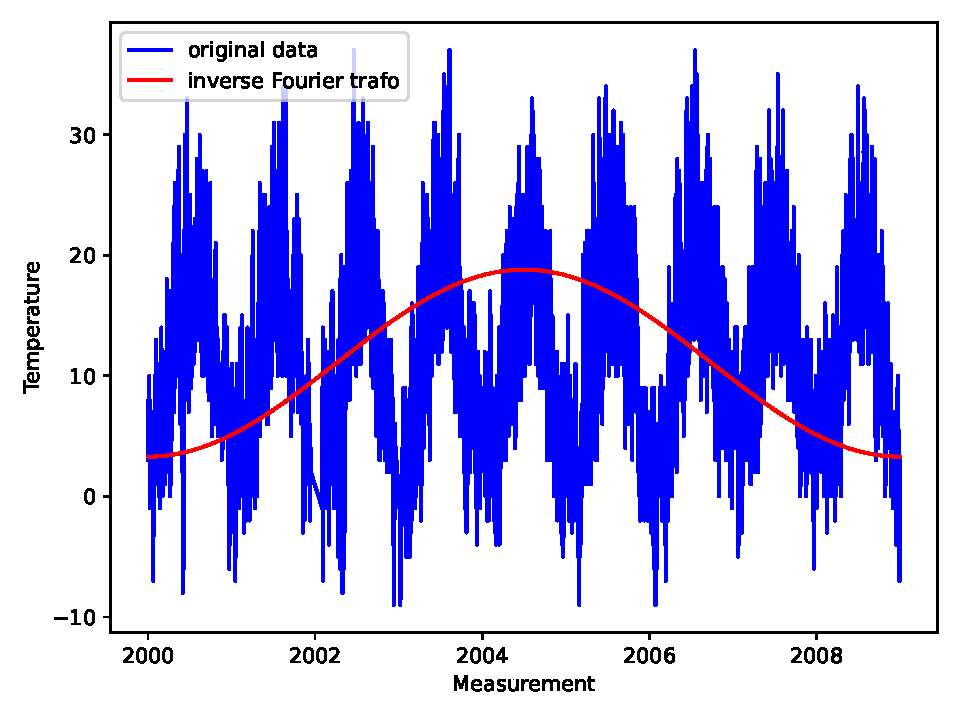
\includegraphics{build/e.pdf}
    \caption{Berechnete Werte für $e_0$}
    \label{fig:e}
\end{figure}

\begin{figure}
    \centering
    \includegraphics{build/e_sortiert.pdf}
    \caption{Berechnete Werte für $e_0$ nach grösse sortiert}
    \label{fig:e_sortiert}
\end{figure}

Nun wird der größte gemeinsame Teiler der Ladungen bestimmt. Aufgrund der Tatsache, dass die gemessenen Werte Fehler haben, ist nicht davon auszugehen, dass alle Ladungen ganze Vielfache voneinander sind.
Deshalb wird der kleinste Teiler gesucht, bei dem die übrigbleibende Differenz unter $\num{1e-19}$ liegt, da bekannt ist, dass die Elementarladung in dieser Größenordnung liegt.
Mit Hilfe dieses Vorgehens wird folgende Ladung  bestimmt:
\begin{equation*}
    e_0 = \qty{2.0(0.5)e-19}{\coulomb}
\end{equation*}

Daraus lässt sich dann noch mit Hilfe der Faraday-Konstante $F = \qty{96485.3321233100184}{\coulomb\per\mole}$ \cite[575]{Metzler}  über
\begin{equation*}
    N_\text{A} = \frac{F}{e_0}
\end{equation*}
die Avogadro-Konstante bestimmen. Diese ergibt sich dann zu:
\begin{equation*}
    N_\text{A} = \qty{4.9(1.3)e+23}{\per\mole}
\end{equation*}